%%%%%%%%%%%%%%%%%%%%% chapter.tex %%%%%%%%%%%%%%%%%%%%%%%%%%%%%%%%%
%
% sample chapter
%
% Use this file as a template for your own input.
%
%%%%%%%%%%%%%%%%%%%%%%%% Springer-Verlag %%%%%%%%%%%%%%%%%%%%%%%%%%

\chapter{Expectation-Maximization (EM)}
\section{Itroduzione}
\'E una tecnica alternativa più robusta per la massima verosomiglianza, essa è utilizzata per stimare le densità di probabilità nel caso di dati mancanti, ovvero i dati per i quali non abbiamo osservazioni. Abbiamo già visto la stima di densità e adesso facciamo una breve panoramica, in particolare riprendiamo gli elementi fondamentali di come si stima la densità, poi verrà spiegata la differenza che intercorre tra un dato osservato ed un dato mancante, e da qui l'algoritmo EM. Cos' è la stima di densità e perché è importante stimarla? L'abbiamo già visto più di una volta, fondamentalmente noi stimiamo la probabilità della classe data l'osservazione $P(w_i | \mathbf{x})$, quindi stimiamo la probabilità a posteriori. Nel pattern recognition è importante perché proprio sulla base delle probabilità a posteriori è possibile effettuare la classificazione. Stimare la densità di probabilità dai dati equivale a conoscere i parametri del modello nel caso parametrico (nota: ma anche quelli non parametrici hanno dei parametri). Lo scopo principale è quello di apprendere i parametri per la macchina che vuole effettuare il riconoscimento. Come funziona la stima della densità? Forniti dei campioni $x_i$, ci sono due filosofie fondamentali, la prima è quella parametrica mentre l'altra è quella non parametrica. La stima della densità mediante metodi parametrici si basa sull'ipotesi che la forma della densità della classe è nota ma non sono noti i parametri di tale forma di densità, per cui la stima riguarda i parametri che meglio modella i dati. Come facciamo a misurare qual'è la distanza che intercorre tra la verosomiglianza realistica e quella che stiamo stimando di volta in volta? Utilizzo la massima verosomiglianza. In questa stima della densità incide molto anche la conoscenza a priori, che potrebbe non incidere se le conoscenze a priori fossero uguali. Invece nel caso non parametrico non facciamo nessuna ipotesi sulla forma di densità di probabilità, per cui il modello si stima direttamente dai dati, facciamo soltanto alcune ipotesi su quanto deve essere grande la regione o il volume che racchiude i punti in modo tale da poter stimare i parametri del modello ed anche se stesso, quindi oltre a stimare i parametri stimo anche il modello stesso. Per fare questo abbiamo visto le finestre di parzen ed il knn. In questo caso la conoscenza a priori è molto meno influente, perché tentiamo di stimare direttamente la densità di probabilità $p(x)$. Nel caso parametrico, nel quale vogliamo stimare la migliore approssimazione del modello parametrizzato rispetto a dati allora utilizziamo la massima verosomiglianza. Il metodo standard si basa sulla formula baesiana ed è applicabile alla stima di densità di probabilità parametrica. La verosomiglianza è la $p(x|\omega)$, quindi la probabilità della $x$ dato la classe. Poiché però il ragionamento si applica ad ogni singola classe, noi non stimiamo la $p(x|\omega)$ ma stimiamo la $p(x)$, ma è equivalente a stimare la $p(x|\omega)$ perchè praticamente lo facciamo classe per classe, quindi la stima di $p(x|\omega)$ la facciamo sulla base dei parametri del modello, ecco perché dalla $p(x|\omega)$ stimiamo la $p(x|\theta)$ e nell'ipotesi delle i.i.d. possiamo dire che questo non è altro che la produttoria per i $p(x_i|\theta)$, dove gli $x_i$ sono i campioni del nostro training set. Come sappiamo alla fine non affrontiamo la verosomigilanza ma affrontiamo la log verosomiglianza o equivalentemente la meno log verosomiglianza, quindi si tende o a massimizzare la log verosomiglianza o a minimizzare la meno log verosomiglianza. Questo equivale a stimare una funzione di errore che andiamo a minimizzare rispetto ai parametri $\theta$, tipicamente facciamo le derivate parziali rispetto ai $\theta$ le poniamo uguali a zero e risolviamo il sistema rispetto a $\theta$. Per la gaussiana in particolare i parametri sono la media e la varianza o la matrice di covarianza nel caso multivariato. Il problema sorge quando i dati sono mancanti, ovvero che l dati sono intrisecamente inaccessibili, ovvero quando non è possibile conoscere intrinsecamente una certa probabilità a posteriori come la $p(\omega|x)$, quindi se non conosco la dimensione del problema, in tal caso il modello non è un modello unico per ogni classe, ma è un modello detto di costellazione quindi un modello campionato, un modello che non rappresenta tutta la classe ma rappresenta parti della classe, in virtù di tutto questo ci sono parti della classe che non sono rappresentative nel training set, ma che invece nel test set lo sono, ma non avendo i dati campioni  per quella parte allora non è possibile stimare la densità di probabilità della classe. Fondamentalmente è intrinsecamente difficile conoscere la densità di probabilità della classe in quanto non sono note parti della densità.\\

\noindent Questo può essere rappresentato come modello di mixture di gaussiane, praticamente la densità di probabilità di classe è una mixtura di gaussiane e le varie parti in cui la classe si suddivide possono essere modellate singolarmente con delle gaussiane, è possibile però che c'è una parte che nel training set non è modellabile, ma che sia ben rappresentata dai dati di test. Quindi quando vengono fuori i dati di test a cui applichiamo il sistema tutto fallisce in quanto non avevamo i dati su cui fare il training. Questo è da un punto di vista probabilistico, invece da un punto di vista proprio di dati è possibile che i dati siano mancanti o anche se presenti siano sbagliati, quindi l'acquisizione è stata effettuata in modo errato. In questo caso quindi abbiamo informazioni  non complete oltre ad avere variazioni dei dati stessi.  Ma se i dati mancanti (quindi quelli che non abbiamo o che sono sbagliati, che è meglio considerare mancanti) sono correlati con quelli osservati, allora possiamo sperare che l'informazione estratta sui dati mancanti possa  derivare da quelli osservati. Quindi se c'è forte correlazione tra i dati mancanti e quelli osservati allora potrebbero bastare quelli osservati, ma se i dati mancanti sono indipendenti da quelli osservati, allora l'informazione è persa e non è possibile recuperare.\\


\section{Algoritmo EM}
\noindent Adesso facciamo un esempio abbastanza rappresentativo, immaginiamo di avere dei dati sui quali stimiamo la nostra $p(y,z|\theta)$ (fig \ref{figEM}), dove $y$ e $z$ sono le variabili casuali e $\theta$ sono i parametri di un modello.
\begin{figure}
\centering
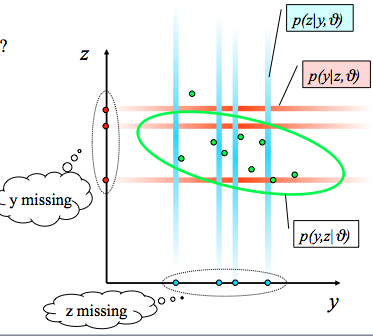
\includegraphics[scale=0.7]{img/figEM.png}
\caption{}
\label{figEM}
\end{figure}
Ipotizziamo di riuscire a stimare una gaussiana congiunta, però è possibile che per alcuni punti che chiamiamo con $x_i$ non abbiamo informazione, quindi sono valori non osservati, o dati mancanti. Come osservato in figura abbiamo due casi: per il primo abbiamo $y$ mancante, mentre per il secondo abbiamo $z$ mancante. A questo punto come possiamo affrontare il problema dei dati mancanti? Potremmo fare un po' di inferenza, per esempio per i dati in blu potremmo stimare la $p(z|y, \theta)$ dato che conosciamo $y$ e $\theta$ che è stato stimato da $p(y,z|\theta)$, quindi possiamo fare questa stima per ciascun dato mancante, lo stesso possiamo farlo dall'altro lato, infatti possiamo stimare $p(y|z, \theta$, quindi possiamo stimare fondamentalmente le singole variabili casuali nota l'altra variabile casuale (in questo caso banalmente uguale a zero). In questo caso semplice noi conosciamo sia $y$ che $z$, inoltre si può stimare una rispetto all'altra considerando che il $\theta$ è lo stesso, quindi visto che ho stimato i parametri $\theta$ sulla distribuzione cerchiata di verde, questi stessi parametri  sono sufficienti per consentire la stima anche delle altre due probabilità? L'idea di EM dice che: se avessimo una stima della densità congiunte, le densità condizionali ci direbbero tutto anche sui dati mancanti. Quindi se io conoscessi la $p(y,z|\theta)$ qualsiasi dato io ho a disposizione o non ho a disposizione, $p(z|y, \theta)$ o la $p(y|z, \theta)$ sarebbe facile da calcolare, perché non sarebbe altro che una marginalizzazione della probabilità congiunta. Vediamo un esempio nel discreto, quindi se ho due variabili casuali e la matrice delle probabilità congiunte $P(x,z)$, per marginalizzare come faccio? Quindi come faccio ad avere $p(x)$ oppure $p(z)$? Sommo riga per riga e ottengo la p(x), sommo colonna per colonna ed ottengo la $p(z)$, questo è quello che accade nel discreto. Adesso stiamo dicendo la stessa cosa soltanto che c'è un problema, ovvero quello che devo conoscere è la $p(y,z)$ che è possibile conoscere soltanto stimando la densità di probabilità, per esempio se diciamo che si tratta di una gaussiana multivariata allora vado a stimare la media e la covarianza con le tecniche che già conosciamo, fondamentalmente non ho $p(y,z)$ ma ho $p(y,z|\theta)$, cioè vado a stimare $\theta$, ma se conoscessi quella reale a quel punto il problema sarebbe facile perché potrei conoscere le probabilità condizionate di ognuna, anche di quelle mancanti. A questo punto se avessimo una stima della distribuzione dei dati mancanti, allora a quel punto potremmo usarla per stimare la densità congiunta. Data una stima della probabilità congiunta riesco a stimare la probabilità condizionata, cioè la $p(y|z)$ o la $p(z|y)$ ed anche per i dati mancanti potrei ricalcolare la $p(y,z)$.  Poteri iterare il procedimento finché l'approssimazione sia abbastanza buona, naturalmente questa stima della densità di probabilità è sempre relativa ai parametri, quindi quando diciamo buona significa che i parametri tra un iterazione e l'altra sono pressoché gli stessi, quindi la differenza è al di sotto di una certa soglia, oppure vado a stimare la densità di probabilità (la bontà) applicando la massima verosomiglianza. \\

\noindent Da qui l'idea di base del'EM. Adesso guardiamo l'aspetto più formale. Stimiamo la $p(y,z|\mu, \Sigma)$, quindi stiamo immaginando una gaussiana. Lo facciamo dai dati disponibili, ovvero da quelli osservati. Adesso vogliamo effettuare una stima a massima verosomiglianza anche se non conosciamo tutti i dati. Se conoscessimo i dati mancanti allora potremmo minimizzare la log verosomiglianza negativa, oppure massimizzare la log verosomiglianza per ottenere la stima. Con la $o$ indichiamo il dato osservato ed $m$ indichiamo il dato mancante
\begin{equation}\label{177}
L_{om}(X|\theta) = - \sum \log p(x_i^o, x_i^m | \theta) \quad \quad \quad \theta = \{\mu, \Sigma\} 
\end{equation}
Quindi potremmo calcolare la verosomiglianza su tutti i dati, sia osservati che quelli mancanti. Siccome però il dato mancante non ce l'ho, come faccio a calcolarlo? Quindi è una densità di probabilità congiunta tra dati mancanti e dati osservati, allora questa stima viene effettuata soltanto sui dati osservati. Come faccio a calcolarmi quelli mancanti? Poiché non conosciamo i dati mancanti $x_i^m$ vogliamo minimizzare la verosomiglianza dei dati osservati quindi
\begin{equation}\label{178}
L_o(x^o | \theta) = - \log p(x^o | \theta) = - \sum_i \log p(x_i^o | \theta)
\end{equation}
la verosomiglianza la calcoliamo soltanto sui dati osservati però poi applico un trucco. $\log p(x_i^o | \theta)$ lo scrivo come la marginalizzazione della probabilità congiunta $p(x^m, x_i^o | \theta)$, e come abbiamo visto prima, la marginalizzazione nel discreto è una sommatoria, quindi nel continuo diventa un integrale, quindi il tutto diventa
\begin{equation}\label{179}
L_o(x^o | \theta) = -\sum_i \log \int p(x^m, x_i^o | \theta) \ dx^m
\end{equation}
In sintesi: Voglio massimizzare la verosomiglianza su tutti i dati, se conoscessi tutti i dati, sia quelli osservati e quelli non osservati allora la verosomiglianza sarebbe la \ref{177}, ma dato che non ho i dati quindi non ho $x_i^m$ e quindi la faccio soltanto per quelli osservati mediante la \ref{178}, ma poi il ragionamento è: dico che la $p(x_i^o | \theta)$ non è altro che la marginalizzazione della probabilità congiunta dei dati mancanti e dei dati osservati quindi la posso scrivere come la \ref{179}.\\

\noindent Adesso però questa soluzione non è che la stimiamo una volta soltanto, ma faccio una procedura di raffinamento, quindi stimo di volta in volta i parametri. Per il momento consideriamo soltanto che sia il logaritmo di un integrale, l'idea è che il processo sia iterativo.  Allora la stima $P_o(x_i^o|\theta)$ la stimiamo in modo iterativo, quindi la chiamiamo $p_n(.)$ per $p(.|\theta_n)$ perché dipende dai $\theta$ parametri calcolati però all'iterazione $n-$esima, quindi fondamentalmente è dipendente dai dati, ma quelli che cambiano sono i parametri della distribuzione di probabilità, quindi il punto sta ad indicare che la variabile non cambia nel passo iterativo, ma quello che cambia iterativamente sono i parametri $\theta_n$. Riscriviamo l'espressione per la verosomiglinaza
\begin{equation}
L_o (\theta_n) = - \log p_n(X^o)
\end{equation}
questi sono i pattern osservati, poi abbiamo meno log verosomiglianza al passo n, a questo punto abbiamo poi marginalizzato quindi scriviamo che $p_n(X^o)$ non è altro che l'integrale \ref{179}, quindi riscrivendo abbiamo $\int p_n(X^o, X^m)$ (per semplicità notazionale evitiamo di prtarci $\theta$), però la probabilità congiunta la posso scrivere come $\int p(X^m | X^o) \ p(X^o) \ dX^m$, quindi otteniamo 
\begin{equation}
L_o (\theta_n) = -\log \int p_n(X^m | X^o) \ p(X^o) \ dX^m
\end{equation}
ma il logaritmo di un integrale è uguale all'integrale dei logaritmi, quindi
%\begin{equation}
%L_o (\theta_n) = - \int \log p_n(X^m | X^o) \ p(X^o) \ dX^m
%\end{equation}
\begin{equation}
L_o (\theta_n) = -\int p_n(X^m|X^o) \log p_n(X^o) \ dX^m
\end{equation}
a questo punto cosa facciamo?  Divido e moltiplico per la stessa quantità 
\begin{equation}
L_o (\theta_n) = -\int p_n(X^m|X^o) \log p_n(X^o) \frac{p_n(X^m | X^o)}{p_n(X^m | X^o)} \ dX^m
\end{equation}
quindi adesso abbiamo un logaritmo di un rapporto e possiamo scriverlo in questo modo
\begin{equation}
L_o (\theta_n) = -\int p_n(X^m|X^o) \left[ \log p_n(X^o) p_n(X^m | X^o) + \log \frac{1}{p_n(X^m | X^o)} \right] \ dX^m
\end{equation}
A questo punto $p_n(X^o) p_n(X^m | X^o) = p_n(X^m, X^o)$ e $\log \frac{1}{p_n(X^m | X^o)} = - \log p_n(X^m | X^o)$ 
sostituendo otteniamo
\begin{equation}
L_o (\theta_n) = -\int p_n(X^m|X^o) \left[ \log p_n(X^m, X^o)  - \log p_n(X^m | X^o) \right] \ dX^m
\end{equation}
effettuando le opportune moltiplicazioni
\begin{equation}
L_o (\theta_n) = -\int p_n(X^m|X^o) \log p_n(X^m, X^o)  - p_n(X^m|X^o) \log p_n(X^m | X^o)  \ dX^m
\end{equation}
per poi arrivare a questa conclusione
\begin{equation}\label{187}
L_o (\theta_n) = -\int p_n(X^m|X^o) \log p_n(X^m, X^o) \ dX^m + \int p_n(X^m|X^o) \log p_n(X^m | X^o)  \ dX^m
\end{equation}
La prima la chiamo $Q(\theta_n, \theta_n)$ e la seconda la chiamo $H(\theta_n)$
ottenendo
\begin{equation}
L_o (\theta_n) = Q(\theta_n, \theta_n) - H(\theta_n)
\end{equation}
Posso dire che $L_o$, ovvero la verosomiglianza sui parametri $\theta_n$ al passo $n$ è uguale ad una funzione $Q$ - un altra funzione $H$ dove $Q$ ed $H$ sono quelle nella \ref{187}.\\

\noindent Adesso possiamo scrivere la stessa anche in un altro modo, come 
\begin{equation}
L_o (\theta_n) = - \log p_n(X^o)
\end{equation}
e come prima marginalizziamo per ottenere
\begin{equation}
L_o (\theta_n) = - \log \int p_n(X^m, X^o) \ dX^m
\end{equation}
ancora una volta, moltiplicando e dividendo per la stessa quantità, però questa volta per scelta utilizziamo $p_{n-1}(X^m, X^o)$ cioè la stima della densità di probabilità al passo precendente 
\begin{equation}
L_o (\theta_n) = - \log \int \frac{p_n(X^m, X^o)}{p_{n-1}(X^m | X^o)} p_{n-1}(X^m | X^o) \ dX^m
\end{equation}
ed usiamo la disequazione di Jensen la quale dice che
\begin{equation}
\log \int a(x) g(x) \ dx \geq \int a(x) \log g(x) \ dx \quad \quad \quad \text{se} \ \int a(x) \ dx = 1
\end{equation}
o equivalentemente moltiplicando semplicemente per $-1$
\begin{equation}
- \log \int a(x) g(x) \ dx \leq - \int a(x) \log g(x) \ dx
\end{equation}
A questo punto dato che 
\begin{equation}
L_o (\theta_n) = - \log \int \frac{p_n(X^m, X^o)}{p_{n-1}(X^m | X^o)} p_{n-1}(X^m | X^o) \ dX^m
\end{equation}
se poniamo $a(x) = p_{n-1}(X^m | X^o)$ e $g(x) = \frac{p_n(X^m, X^o)}{p_{n-1}(X^m | X^o)}$,
per la disequazione di Jensen $ \leq - \int a(x) \log g(x) \ dx$ abbiamo che
\begin{equation}
L_o (\theta_n) \leq - \int p_{n-1}(X^m | X^o) \ \log \frac{p_n(X^m, X^o)}{p_{n-1}(X^m | X^o)} \ dX^m
\end{equation}
semplifichiamo per le proprietà dei logaritmi
\begin{equation}
L_o (\theta_n) \leq - \int p_{n-1}(X^m | X^o) \left[ \log p_n(X^m, X^o) - \log p_{n-1}(X^m | X^o) \right] \ dX^m
\end{equation}
\begin{equation}
L_o (\theta_n) \leq - \int p_{n-1}(X^m | X^o) \log p_n(X^m, X^o) -  p_{n-1}(X^m | X^o) \log p_{n-1}(X^m | X^o) \ dX^m
\end{equation}
\begin{equation}
L_o (\theta_n) \leq - \int p_{n-1}(X^m | X^o) \log p_n(X^m, X^o) \ dX^m + \int p_{n-1}(X^m | X^o) \log p_{n-1}(X^m | X^o) \ dX^m
\end{equation}
e questa volta invece abbiamo due funzioni $Q$ e $H$ come mostrato
\begin{equation}
L_o (\theta_n) \equiv Q(\theta_{n-1}, \theta_n) - H(\theta_{n-1})
\end{equation}
Allora a questo punto dobbiamo minimizzare la log verosomiglianza negativa, quindi minimizzare una quantità negativa equivale a minimizzare la $Q$, visto che 
\begin{equation}
L_o (\theta_{n-1}) = Q(\theta_{n-1}, \theta_{n-1}) - H(\theta_{n-1})
\end{equation}
allora minimzzo $Q$, sostituisco il valore per cui ho minimizzato $Q$ sottraggo $H(\theta_{n-1})$, ma questa sarà sicuramente maggiore o uguale di $L_o(\theta_n)$ quindi
\begin{equation}
L_o (\theta_n) \leq Q(\theta_{n-1}, \theta_n) - H(\theta_{n-1})
\end{equation}
Immaginiamo di mettere sull'asse delle ascisse i valori di $\theta$ (fig \ref{em2})
\begin{figure}
\centering
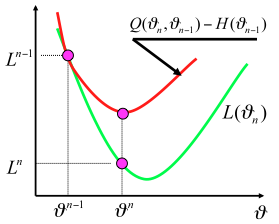
\includegraphics[scale=0.7]{img/em2.png}
\caption{}
\label{em2}
\end{figure}
e che la log verosomiglianza sia quella di colore verde, adesso voglio cercare il minimo di questa log verosomiglianza negativa. Dove trovare il minimo? Nel parametro $\theta_n$. Supponiamo però che mi trovi al paramentro $\theta_{n-1}$ ed il valore di questa verosomiglianza negativa sia $L^{n-1}$, voglio trovare il valore $\theta_n$ per cui $L_n$ assuma un valore più basso rispetto ad $L^{n-1}$, quindi certamente $L_o(\theta_n) \leq L_o(\theta_{n-1})$, quindi il procedimento iterativo deve far si che i parametri che trovo, migliorano la log verosomiglianza negativa, cioè trovino un valore della log verosomiglianza sempre più basso.  Voglio trovare un altro parametro $\theta_n$ per cui la log verosomiglianza mi diventi più bassa, quindi $L^n \leq L^{n-1}$ ma $L^{n-1}$ la posso scrivere come $Q(\theta_n, \theta_{n-1}) - H(\theta_{n-1})$, quindi questa dovrebbe essere $ \geq L^n$, se non cambio niente della funzione $H$, quindi la lascio inalterata, allora minimizzare la log verosomiglianza equivale a minimizzare la $Q$ introducendo naturalmente la $Q$ che non si basa soltanto sul $\theta_{n-1}$ ma sia su $\theta_{n}$ che $\theta_{n-1}$. \\

\noindent Fondamentalmente mostra che se minimizziamo la $Q(\theta)$ rispetto al secondo argomento la verosomiglianza può soltanto aumentare, cioè se minimizzo la Q, un valore più piccolo meno $H(\theta_{n-1})$ non può che portare un valore più alto della log verosomiglianza negativa.\\

\noindent Ripetiamo il concetto: allora dalla prima formulazione abbiamo detto che 
\begin{equation}
L_o (\theta_n) = Q(\theta_{n}, \theta_n) - H(\theta_{n})
\end{equation}
dalla seconda formulazione  abbiamo anche
\begin{equation}
L_o (\theta_n) \leq Q(\theta_{n-1}, \theta_n) - H(\theta_{n-1})
\end{equation}
adesso guardiamo al passo $n-1$ e quindi scriviamo la prima al passo $n-1$ quindi otteniamo
\begin{equation}
L_o (\theta_{n-1}) = Q(\theta_{n-1}, \theta_{n-1}) - H(\theta_{n-1})
\end{equation}
Sicuramente al passo $n$ non faccio altro che diminuire la log verosomiglianza negativa, perché sto iterando, quindi sto trovando dei parametri tale che minimizzo la log verosomiglianza negativa. Per minimizzare la log verosomiglianza devo minimizzare la $Q$, perchè la $H$ resta inalterata. Questo mostra che se vado a minimizzare la $Q$ rispetto al secondo argomento, allora la verosomiglianza può soltanto aumentare, allora abbiamo necessità di mostrare che dopo la convergenza (al valore più basso di $Q$), abbiamo raggiunto il minimo della veromiglianza. In sintesi ad ogni iterazione è necessario minimizzare la seguente espressione,  quindi la $Q$ rispetto a $\theta_n$
\begin{equation}
-\int p_n(X^m|X^o) \log p_n(X^m, X^o) \ dX^m
\end{equation}
questa equivale all'integrale della log probabilità congiunta tra i dati osservati ed i dati mancanti moltiplicato per il valor medio della probabilità congiunta dei dati osservati e dei dati mancanti.\\

\noindent Quindi l'idea è, mi calcolo la stima di densità probabilità congiunta, mi calcolo la probabilità condizionata che viene usata per mediare la densità di probabilità congiunta al passo successivo, e quindi itero successivamente, quindi voglio minimizzare l'aspettazione, quindi stiamo minimizzando il valore atteso della verosomiglinza della probabilità congiunta dove il peso di questa media è calcolato come probabilità condizionate sulla densità di probabilità congiunta del passo precedente. Nel secondo passo dice: Se avessimo la stima della distribuzione dei dati mancanti, quindi stimata la log verosomiglianza su tutti i dati compresi quelli mancanti non faccio altro che fare una stima dei dati mancanti data la distribuzione di probabilità congiunta. E come faccio a fare questo? Marginalizzando rispetto ai dati mancanti.\\

\noindent Adesso se io ho la $p(y,z|\theta)$, quindi ho una stima della densità di probabilità congiunta, allora a questo punto vado a calcolare la probabilità condizionata dei pattern mancanti dato i pattern noti, cioè fondamentalmente se ho stimato la $p(X^m, X^o)$  allora vado a trovare la $p(X^m | X^o)$, quindi prendo questa e la uso per calcolare la probabilità congiunta al passo successivo, quindi ad ogni passo stimo la densità di probabilità congiunta, mi calcolo la probabilità condizionata e la riuso nella successiva, quindi stimo la densità di probabilità congiunta del passo E, la uso poi per calcolare la probabilità condizionata $p(X^m|X^o)$ con i parametri del passo precedente. Quindi faccio una stima delle densità probabilità congiunte utilizzando le probabilità condizionate come medie della log verosomoglianza, fatto questo stimo la densità di probabilità condizionata del pattern mancanti dati i pattern osservati per ristimare di nuovo le densità di probabilità congiunta ed itero questi due passi fintanto che o ho raggiunto un numero di passi ben definito oppure le due stime di $\theta$ al passo $n$ ed al passo $n-1$ si differiscono di poco.

%
